\documentclass[border = 5mm]{standalone}
%\documentclass[dvisvgm]{minimal}

\usepackage{tkz-euclide}

\usepackage[OT1]{fontenc}
\usepackage{sansmathfonts}

\begin{document}
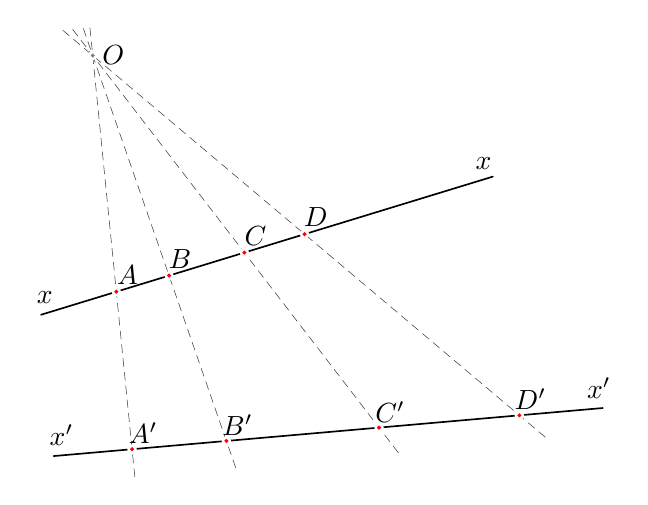
\begin{tikzpicture}
		
% Point O
\tkzDefPoint(-.5,5){O}

% Draw line x with A, B, D, and D
\tkzDefPoint(-.2,2){A}
\tkzDefShiftPoint[A](17:0.7){B}
\tkzDefShiftPoint[B](17:1){C}
\tkzDefShiftPoint[C](17:0.8){D}

\tkzDrawLine[add = 0.4 and 1, semithick](A,D)
	
% Draw line x'
\tkzDefPoint(0,0){X}
\tkzDefShiftPoint[X](5:5){Y}
\tkzDrawLines[add = 0.2 and 0.2, semithick](X,Y)

% Intersections of projection lines with x
\foreach \i\j in {A/A', B/B', C/C', D/D'} {
\tkzInterLL(O,\i)(X,Y) \tkzGetPoint{\j}
}

% Draw projection lines
\tkzDrawLines[gray!150, add = 0.07 and 0.07, densely dashed, very thin](O,A' O,B' O,C' O,D')

% Label points and lines
\tkzDrawPoints[color=white, size=3](A,B,C,D,A',B',C',D',O)
\tkzDrawPoints[color=red, size=1](A,B,C,D,A',B',C',D') 
\tkzDrawPoints[color=gray, size=1](O)

\tkzLabelPoints[xshift=4, yshift=13](A,B,C,D,A',B',C',D') {A,B,C,D,A',B',C',D'}
\tkzLabelPoints[right](O){O} 

\tkzLabelLine[pos=-0.38, above](A,D){$x$}     
\tkzLabelLine[pos=1.95, above](A,D){$x$}
\tkzLabelLine[pos=-0.18, above](X,Y){$x'$}  
\tkzLabelLine[pos=1.19, above](X,Y){$x'$}

\end{tikzpicture}
\end{document}
